\documentclass[conference]{IEEEtran}

%\IEEEoverridecommandlockouts
% The preceding line is only needed to identify funding in the first footnote. If that is unneeded, please comment it out.

\usepackage{cite}
\usepackage{amsmath,amssymb,amsfonts}
\usepackage{algorithmic}
\usepackage{graphicx}
\usepackage{grffile}
\usepackage{textcomp}
\usepackage{xcolor}
\usepackage{url}
\usepackage{longtable}
\usepackage{tabularx,booktabs}
\usepackage{array}
\newcolumntype{P}[1]{>{\centering\arraybackslash}p{#1}}
\newcolumntype{M}[1]{>{\centering\arraybackslash}m{#1}}
\newcolumntype{C}{>{\centering\arraybackslash}X}

\usepackage[section]{placeins}
\def\BibTeX{{\rm B\kern-.05em{\sc i\kern-.025em b}\kern-.08em
    T\kern-.1667em\lower.7ex\hbox{E}\kern-.125emX}}

\graphicspath{{C:/Users/Admin/Desktop/CSC/DataPic/}}

% Title 
\title{\textbf{Lightweight Symmetric Cryptography Algorithm Efficiency on IoT Devices}}
%{\footnotesize \textsuperscript{*}Note: Sub-titles are not captured in Xplore and
%should not be used}
%\thanks{Identify applicable funding agency here. If none, delete this.}
%}
\author{\IEEEauthorblockN{Tran Ngoc Bao Huynh}
\IEEEauthorblockA{California State University - Sacramento\\ 
	Sacramento, CA, United State\\
	tranngocbaohuynh@csus.edu}
\and
\IEEEauthorblockN{Jericho Rivero}
\IEEEauthorblockA{California State University - Sacramento\\
	Sacramento, CA, United State\\
	jerichorivero@csus.edu}
\and
\IEEEauthorblockN{Angelica Smith-Evans}
\IEEEauthorblockA{California State University - Sacramento\\
	Sacramento, CA, United State\\
	angelicasmith-evans@csus.edu}
\and
\IEEEauthorblockN{Ong Thao}
\IEEEauthorblockA{California State University - Sacramento\\
	Sacramento, CA, United State\\
	ongthao@csus.edu}
\and
\IEEEauthorblockN{Yuan Cheng}
\IEEEauthorblockA{California State University - Sacramento\\
	Sacramento, CA, United State\\
	yuan.cheng@csus.edu}
}

% Keywords command
\providecommand{\keywords}[1]
{
	\small
	\textbf{\textit{Keywords---}}#1
}

% Paper
\begin{document}

\maketitle

\begin{abstract}
\textmd{\textit{We analyzed the performance of multiple Symmetric cryptographic ciphers on an Internet of Things device. Our intention was to reveal which of these algorithms performed the most efficiently on a constrained device. We gathered data for each algorithm’s performance through three metrics: throughput, power consumption, and time taken from encryption to decryption of data. We discovered that amongst our chosen ciphers, CHACHA20 is a great option for encrypting/decrypting on a constrained device.}}
\end{abstract}

\keywords{\textit{Lightweight encryption, lightweight block ciphers, lightweight stream ciphers, IoT, Internet of Things.}}

\section{Introduction}
Apple watches, Google Home, and Samsung refrigerators are examples of a technology that we call “Internet of Things” (IoT). These devices are connected to the internet and gives them the ability to collect data, transfer data, and interact with one another. The compactness of these devices means that they are more portable than your average computer but definitely less powerful. With the devices being less powerful and being abundant, they are more likely to be compromised by attackers. While the obvious solution is to implement cryptographic algorithms on these devices, doing so would not be an easy feat considering the resources that these devices have access to.
In this project, we compare and analyze the performance capabilities of different lightweight encryption algorithms on an IoT device. The purpose of our project is to identify which encryption algorithm is best suited to encrypt and decrypt data on an IoT device. Because of the nature of IoT devices, it is especially important to have efficiency and low power consumption. 
We preface our experimentation by explaining our own definition of the Internet of Things. This is to establish our scope. Moving on, we talk about the necessity for lightweight encryption algorithms on these devices. Then, we explain the reasoning behind our chosen algorithms, as well as provide background information on these algorithms. Next, we explain our testing methodology. We discuss the pieces of hardware we chose for testing, as well as other tools prevalent to our data gathering. Moving on, we explain the results of the experiment, and consider areas in which our testing was limited. Finally, we synthesize the results of the testing to make our claim about which method of encryption is the most efficient.

\section{Background}
In the following section, we discuss our definition of the Internet of Things. Afterwards, we describe lightweight symmetric encryption ciphers and their relevance to IoT devices. Further, we describe the algorithms chosen for this experimentation.	

\subsection{Internet of Things}
The Internet of Things is a developing field of technology, which synergizes many fields, including telecommunications, informatics, electronics, and social science. The Internet of Things describes any interconnection of low-resource devices. In our research, the Internet of Things is a broad term which is only characterized by the use of these low-resource devices. Examples of which could be microcontrollers such as the ESP32, ESP8266, or Arduino. These devices have the capability to regulate freezer temperature inside one’s house through their mobile phone. However, these devices pose a huge problem.
Those who are security-conscious would be reluctant to trust IoT devices, because without proper security, sensitive data will easily be compromised. For many IoT devices, communication between devices is wireless. Eavesdropping in this scenario is easy for an attacker.\cite{3} Because of this, IoT requires a way to safely and efficiently secure its data to ensure its longevity. However, because IoT devices are often small and lack resources, methods of security should also require relatively low resources. Therefore, lightweight cryptography would be the best method to secure the traffic of IoT devices.

\subsection{Lightweight Cryptography: State of the Art}
Lightweight cryptography is an algorithm designed to be implemented in constrained environments, such as RFID tags, sensors, and contactless smart cards. Lightweight cryptography takes into consideration the size and power consumption of the hardware to determine lightweight properties. On the software side, a smaller code and/or RAM consumption size is preferable for lightweight applications. Security is not a trade-off, as lightweight cryptography still offers sufficient security. We are particularly interested in symmetric key cryptography. Public key cryptography currently requires resources that are much larger than that of symmetric. Therefore, public key cryptography is not suitable for efficient lightweight implementations.\cite{1}
Lightweight cryptography is considered a requirement for Internet of Things devices. IoT devices demand efficiency in their end-to-end communication. Because these devices are low-resource, any cryptographic algorithm run on the device should take a limited amount of energy. For symmetric key algorithms in particular, the demand for resources is lower for the end devices. Finally, compared to conventional cryptography, lightweight cryptography has a smaller footprint.\cite{1} 

\subsection{Symmetric Cryptography}
Symmetric key cryptography can be separated into three sub-categories: block ciphers, stream ciphers, and hash functions. We do not address hash functions in this report. The development of these lightweight dedicated hash functions has just started and are currently still immature to adopt. \cite{2} We instead focus on block ciphers and stream ciphers to report efficiency. We work with [x block ciphers] and [y stream ciphers]. Below, we give terse information about these algorithms.
AES: AES is a block cipher algorithm with three types of keys: 128 bits, 192 bits, 256 bits. These keys are used for both encryption and decryption. AES has 10, 12, and 14 rounds respectively to key size \cite{4}.   
CLEFIA: CLEFIA is a lightweight block cipher developed by Sony. This algorithm was designed for high efficiency.[3] The ISO/IEC 29192-2 is the current standardization project of lightweight properties. This standard specifies that CLEFIA is a suitable lightweight block cipher for lightweight cryptography implementations.
PRESENT: PRESENT is a lightweight block cipher algorithm with either 80 or 128 bit key [6]. The block length for both keys is 64 bits. 
Both PRESENT and CLEFIA are lightweight block ciphers proposed and under consideration in ISO/IEC 29192-2 \cite{3}.
CHACHA20: CHACHA20 is a stream cipher with 256 bit key and 96 bit IV (initialize vector). CHACHA20 is safe from cache-timing attacks since it uses no table lookups \cite{6}.  

\section{Methodology}
In this section, we will discuss our methodology of the experiment. We describe our methodology in three sections: software utilized, hardware utilized, and data. Our experiment analysed three different metrics, which are: timing analysis from encryption to decryption, throughput, and power consumption. In order to gather this data, we needed a full range of hardware and software tools. Finally, in order to fully realize the power of the ciphers chosen for the experiment, we needed a sufficient data set. 

\subsection{Software Utilized}
We used the OpenSSL library ver 1.1.1 to run available cipher algorithms. Any additional testing was developed using C code. All tests were run on Raspbian OS ver. 4.1, which is based on Debian optimized for the Raspberry Pi.

\subsection{Hardware Utilized}
The IoT device that is currently one of the most powerful while maintaining a compact size is the Raspberry Pi Model 4B. In addition, it is an economical option for IoT implementations. Released in 2019, the R.Pi 4B utilizes a Quad-core 64-bit ARM-Cortex A72 CPU @ 1.5 GHz. It has 4GB RAM available. We are using a 32GB microSD for disk memory, of which 4GB is dedicated to the OS. We recorded this Pi to be operating at around 5V, and ran on average 0.65A during our observation period. The typical operating temperature of this microcomputer handles from 0 to 50 degrees Celsius. During our observation period, the Pi ran at approximately 32±1 degrees Celsius. We did not notice significant changes in temperature through the device while running any tests.
Additionally, we recorded our power consumption data on the MakerHawk USB 3.0 Digital USB multimeter tester. This multimeter is able to measure up to a 4-bit accuracy on the voltage, current, capacity, energy, and power. In addition, this device has an on-board temperature sensor. This device can make measurements when it is in series with the Raspberry Pi’s power supply cable.

\subsection{Average Time and Throughput Data Sets}
For our experiment, we analyzed the average time and throughput for how long it takes to encrypt and decrypt a set of files. Before running encryption and decryption, we first gathered 50 total .WAV files then ran encryption and decryption on the first 25 .WAV files. After compiling a list of working data for the first set of data, we then ran encryption and decryption on the second set of .WAV files. The second set was 484.2MiB smaller than the first set of files. This was done to test the ciphers on two different sizes of data. Our idea was to analyze if performance was proportional to data set size.
In addition to testing on two different sets of .WAV files, we also ran the ciphers on smaller sets of data including one, two, five, and ten files to see how the encryption time and throughput differs with smaller sets of data. However, we decided to not include the smaller data set results since we found that the larger sets of data more closely captures the true average time and throughput than smaller sets of data.

\subsection{Power Consumption Data Sets}
In addition to analyzing average time and throughput, we also gathered data on how much power was being consumed when an algorithm was being run on the IoT device. To determine the power consumed when running the algorithms, we ran each algorithm 20 times, and averaged this data. Each data point would have the peak power consumption subtracted from the idle power consumption. The idle power consumption, which is when the Pi was not running any active processes, averaged at 3.00 Watts. Running the code 20 times in a row on 1 process allows us to record the power consumption by hand much easier. This was important to us because the multimeter used in the experiment sampled several times per seconds. Data gathering could be negatively affected by a misread on miniscule changes in power consumption.

\section{Experiment}
\subsection{Average Time of Encryption and Decryption}
After collecting the data and observing several sets of the compiled data we found that AES-CTR-128 generally did the best in terms of performance for larger and smaller datasets. However, still as seen in Fig. 1 and Fig. 2, we saw that it was hard to see a drastic difference in performance between the modes of operations. Additionally, 3DES actually did better than what we had assumed, especially 3DES-ECB.

\FloatBarrier
\begin{figure}[htbp]
	\centerline{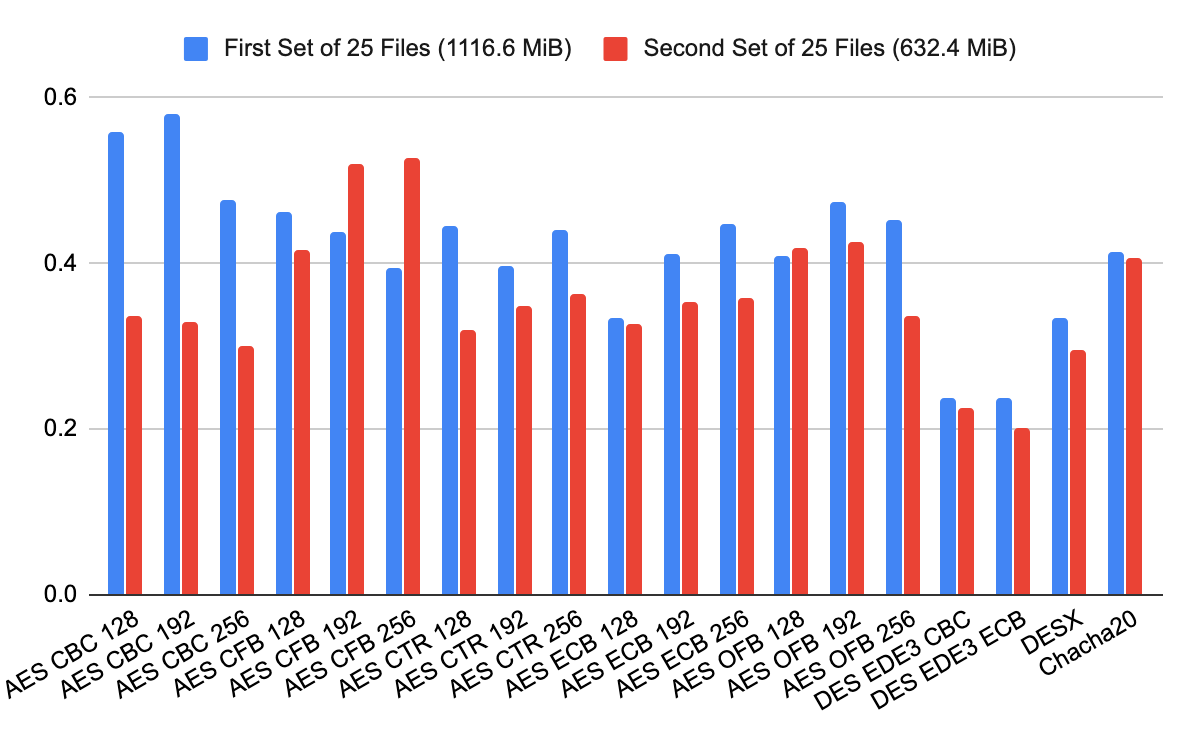
\includegraphics[scale=0.3]{fig1.png}}
	\caption{\textit{In this bar graph, we calculated the average encryption time of two real-time data sets containing 25 files each. As seen from the results, 3DES did better than what we had expected and the performance between the different modes of operations for AES differed.}}
	\label{fig1}
\end{figure}

\begin{figure}[htbp]
	\centerline{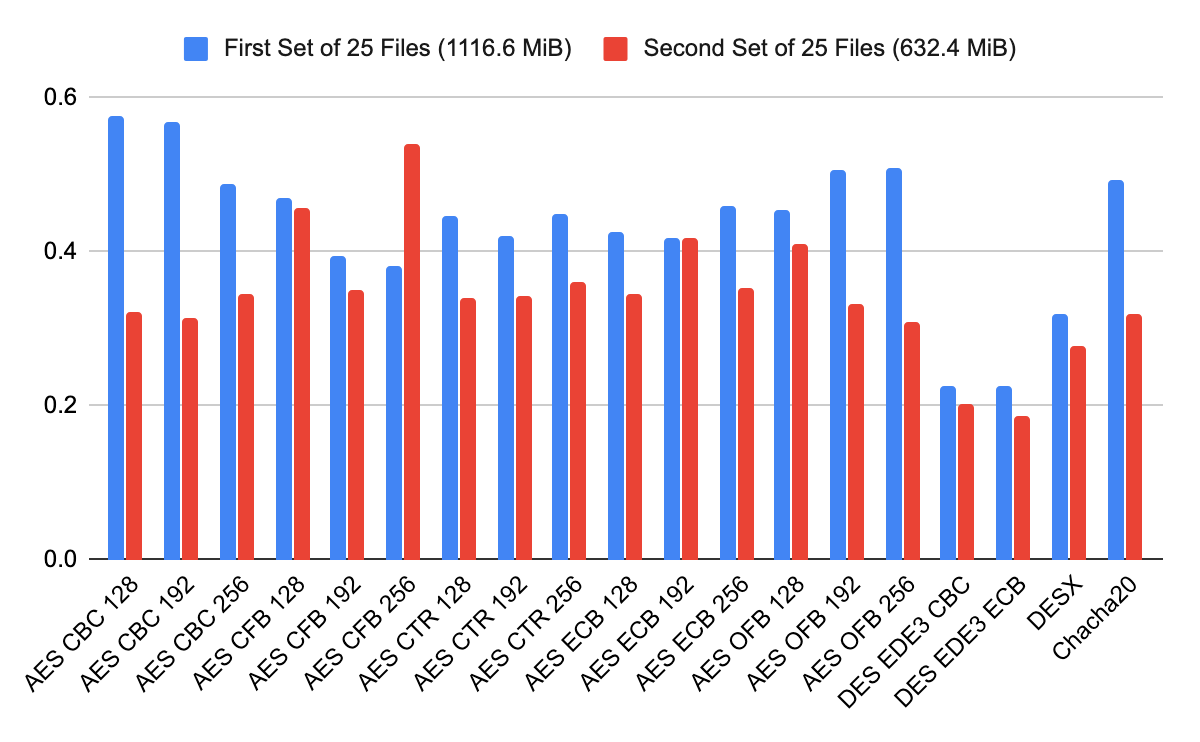
\includegraphics[scale=0.3]{fig2.png}}
	\caption{\textit{For this bar graph, we calculated the average decryption time of the same real-time data sets in Fig 1. From this graph, we see that the results are fairly similar to Fig 1 which is expected as decryption is just encryption but reversed}}
	\label{fig2}
\end{figure}
\FloatBarrier

\subsection{Throughput Analysis}
We calculated the throughput by dividing the total file size (summation of all the individual file sizes) by the encryption and decryption elapsed time. Table 1 and Table 2 in Appendix 1 shows the results of encryption and decryption throughput, respectively. From the calculated data, we find that the second set of 25 files dataset has the best throughput which is reasonable, hence we are encrypting a more reasonable amount of data in less time. 

\subsection{Power Consumption Results and Analysis}
After gathering the power consumed on each algorithm, we saw that PRESENT $64\_128$ consumed the least amount of power out of all of the algorithms we have tested.We also found that PRESENT $64\_128$ has better hardware performance compared to other algorithms in frequency, throughput, and technology\cite{1}. However, PRESENT $64\_128$ has a small gate and block size which makes its security limited. ChaCha20 is the second best in terms of power consumption, trailing behind by approximately 0.05W. Our assumption is that AES-CTR would have the best average encryption time and throughput given that AES is a lightweight algorithm and CTR is the most efficient mode of operation. 

\FloatBarrier
\begin{figure}[htbp]
	\centerline{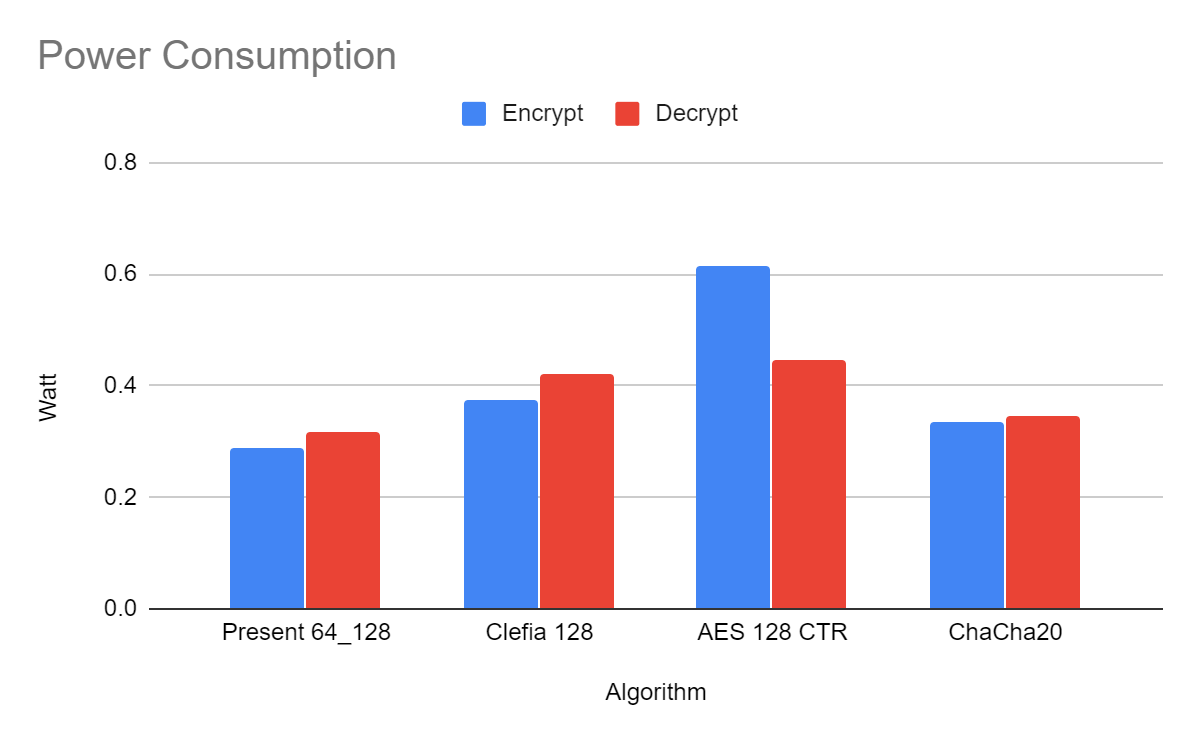
\includegraphics[scale=0.3]{fig3.png}}
	\caption{\textit{This bar graph shows the power consumption by subtracting the peak power consumed during testing from the idle state power consumed (3.000 W) of each cipher algorithm}}
	\label{fig3}
\end{figure}

\begin{figure}[htbp]
	\centerline{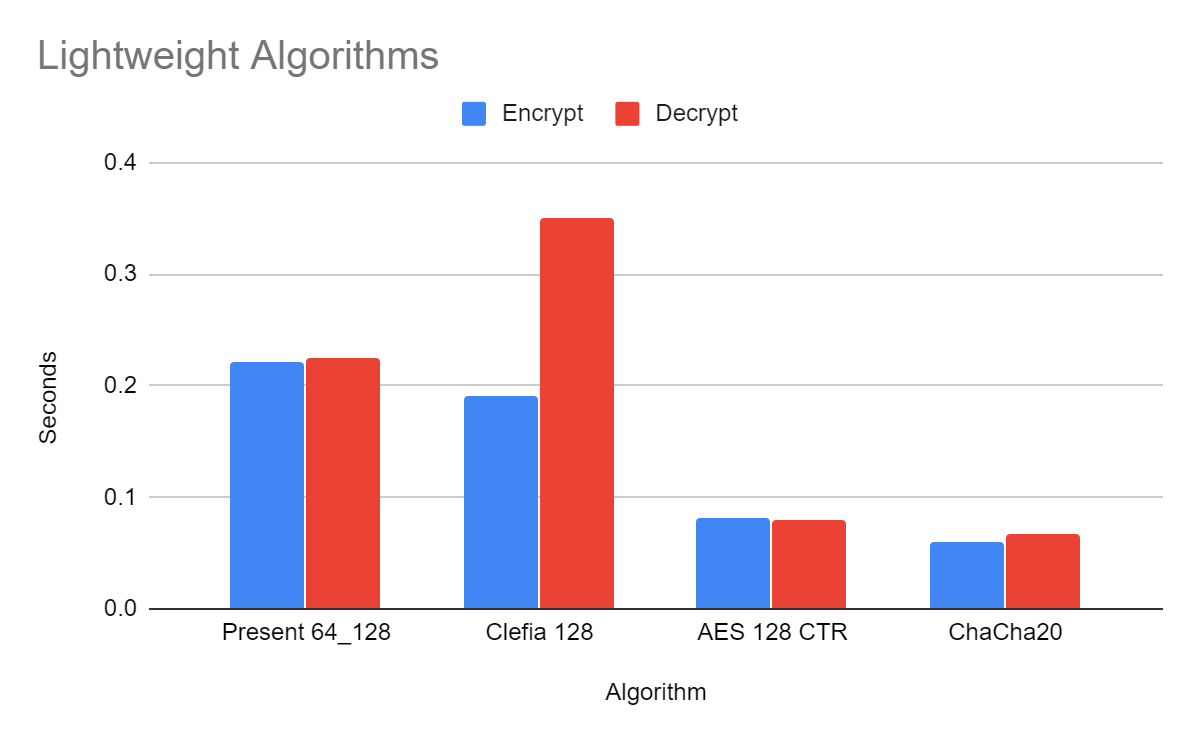
\includegraphics[scale=0.3]{fig4.png}}
	\caption{\textit{This bar graph shows the run-time for both encryption and decryption for the different CHACHA20 Outperforms the other lightweight algorithms.}}
	\label{fig4}
\end{figure}
\FloatBarrier

\subsection{Limitations}
Due to our time limitation and a lack of available resources, we were unable to fully implement other fascinating algorithms of lightweight cryptography. Unfortunately, there are sparse online implementations of ciphers of interest. This is due to an emerging field of study, as well as a necessity to protect intellectual properties. Our collective skill level and lack of resources barred our team from being able to create such algorithms from hand.
In addition to this, our testing was severely handicapped by the Stay-in-Place order that has taken effect during our term. Because of the nature of the COVID-19 pandemic, our team’s progress was impeded by an inability to meet in person or utilize on-campus resources. 
Finally, the scope of our project changed with our own growth and understanding of IoT and the importance of lightweight encryption. Therefore, we were unable to implement some pieces of hardware in our time frame.
In the future, we hope that our research can provide insight as to why certain algorithms are better suited for IoT than others. 

\section{Conclusion}
Our team attempted to confidently claim which, of the cryptographic algorithms available, which is the most efficient. Efficiency is made of three criteria: throughput, length of time from encryption to decryption, and finally power consumption. In terms of trade-off between these three metrics, the ChaCha20 cipher seems to be the clear winner in terms of efficiency on the Raspberry Pi 4B. While PRESENT$64\_128$ seems to trump ChaCha20 in power efficiency, it is not able to execute code nearly as quickly as ChaCha20. The difference between execution time of these algorithms is nearly 1.5 seconds. In terms of usability, that 1.5 seconds of execution is not ideal. To our surprise, any version of the AES block cipher did not trump the other ciphers in any of the metrics. Our research shows that while some ciphers did perform better than others in a single metric, ChaCha20, a stream cipher, seems to be the best all-round implementation of lightweight cryptography on the Raspberry Pi 4GB. We believe this research implies that implementations on other similarly powerful IoT devices will yield similar results.

\section*{Appendix}
\subsection{Data Tables}
\FloatBarrier
\begin{table*}[htbp]
	\begin{center}
		%\scalebox{1}{
		\caption{\textbf{Throughput of Encryption}}
		\begin{tabularx}{\textwidth}{@{}l*{19}{C}c@{}}
			\hline
			%\multicolumn{7}{|c|}{\textbf{Throughput of Encryption}} \\ 
			\toprule
			File Size (MiB) & 1 File (26.9 MiB) & 2 Files (54.6 MiB) & 5 Files (167.5 MiB) & 10 Files (391.1 MiB) & 1st Set of 25 Files (1116.6 MiB) & 2nd Set of 25 Files (632.4 MiB) \\
			
			\midrule
			AES CBC 128  & 42.496 & 19.869 & 16.678 & 14.388 & 13.952 & 8.383 \\
			AES CBC 192  & 34.399 & 21.320 & 15.483 & 14.233 & 14.482 & 8.222 \\
			AES CBC 256  & 14.084 & 18.328 & 14.961 & 13.868 & 11.914 & 7.492 \\
			AES CFB 128  & 34.531 & 40.474 & 11.545 & 13.900 & 11.573 & 10.401\\
			AES CFB 192  & 28.739 & 10.827 & 20.225 & 13.426 & 10.974 & 12.995\\
			AES CFB 256  & 32.685 & 17.687 & 12.215 & 10.508 & 11.288 & 7.478 \\
			\addlinespace
			AES CTR 128  & 45.286 & 37.397 & 22.327 & 12.488 & 11.140 & 7.972 \\
			AES CTR 192  & 21.781 & 10.610 & 9.504  & 12.644 & 9.896  & 8.698 \\
			AES CTR 256  & 42.031 & 44.901 & 15.754 & 13.924 & 11.001 & 9.088 \\
			AES ECB 128  & 43.954 & 46.988 & 22.870 & 13.589 & 8.362  & 8.163 \\
			AES ECB 192  & 36.649 & 18.121 & 35.397 & 12.331 & 10.272 & 8.839 \\
			AES ECB 256  & 37.622 & 10.742 & 11.580 & 11.043 & 11.206 & 8.931 \\
			\addlinespace
			AES OFB 128  & 45.059 & 49.234 & 7.889  & 11.677 & 10.219 & 10.465\\
			AES OFB 192  & 39.099 & 41.239 & 29.552 & 11.675 & 11.870 & 10.619\\
			AES OFB 256  & 37.258 & 27.178 & 18.523 & 13.947 & 11.325 & 8.411 \\
			\addlinespace
			DES EDE3 CBC & 9.036  & 7.392  & 8.796  & 8.296  & 5.924  & 5.628 \\
			DES EDE3 ECB & 8.797  & 9.046  & 7.658  & 6.697  & 5.909  & 5.015 \\
			DESX         & 12.030 & 11.193 & 8.951  & 8.896  & 8.352  & 7.375 \\
			CHACHA20     & 17.826 & 19.389 & 7.376  & 12.101 & 10.327 & 10.147\\
			
			\bottomrule
			\hline
		\end{tabularx} %}
	\end{center}
\end{table*}

\begin{table*}[htbp]
	\begin{center}
		%\scalebox{1}{
		\caption{\textbf{Throughput of Decryption}}
		\begin{tabularx}{\textwidth}{@{}l*{19}{C}c@{}}
			\hline
			%\multicolumn{7}{|c|}{\textbf{Throughput of Encryption}} \\ 
			\toprule
			File Size (MiB) & 1 File (26.9 MiB) & 2 Files (54.6 MiB) & 5 Files (167.5 MiB) & 10 Files (391.1 MiB) & 1st Set of 25 Files (1116.6 MiB) & 2nd Set of 25 Files (632.4 MiB) \\
			
			\midrule
			AES CBC 128  & 46.783 & 50.556 & 22.529 & 18.260 & 14.429 & 8.057 \\
			AES CBC 192  & 49.631 & 48.969 & 41.297 & 17.684 & 14.211 & 7.824 \\
			AES CBC 256  & 38.929 & 42.790 & 17.530 & 17.732 & 12.194 & 8.613 \\
			AES CFB 128  & 48.556 & 14.391 & 21.351 & 13.975 & 11.758 & 11.402\\
			AES CFB 192  & 42.362 & 44.282 & 22.095 & 12.177 & 9.836  & 8.781 \\
			AES CFB 256  & 32.685 & 17.687 & 12.215 & 10.508 & 11.288 & 7.478 \\
			\addlinespace
			AES CTR 128  & 51.731 & 56.231 & 19.182 & 10.148 & 11.159 & 8.497 \\
			AES CTR 192  & 46.946 & 49.367 & 22.115 & 12.174 & 10.527 & 8.567 \\
			AES CTR 256  & 43.811 & 45.236 & 34.163 & 13.745 & 11.253 & 9.017 \\
			AES ECB 128  & 39.793 & 49.189 & 15.670 & 11.183 & 10.618 & 8.641 \\
			AES ECB 192  & 36.649 & 18.121 & 35.397 & 12.331 & 10.272 & 8.839 \\
			AES ECB 256  & 41.131 & 39.394 & 11.749 & 11.602 & 11.504 & 8.814 \\
			\addlinespace
			AES OFB 128  & 50.851 & 50.416 & 15.922 & 11.892 & 11.335 & 10.233\\
			AES OFB 192  & 26.581 & 45.349 & 23.509 & 14.302 & 12.639 & 8.287 \\
			AES OFB 256  & 41.641 & 40.686 & 12.977 & 13.218 & 12.715 & 7.726 \\
			\addlinespace
			DES EDE3 CBC & 9.363  & 9.065  & 7.514  & 8.453  & 5.616  & 5.063 \\
			DES EDE3 ECB & 8.922  & 8.765  & 6.824  & 7.873  & 5.657  & 4.646 \\
			DESX         & 16.698 & 12.179 & 11.840 & 9.224  & 8.001  & 6.949 \\
			CHACHA20     & 77.077 & 82.602 & 13.649 & 11.246 & 12.356 & 7.954 \\
			\bottomrule
			\hline
		\end{tabularx} %}
	\end{center}
\end{table*}
\FloatBarrier

\subsection{A Sample Pictures of Hardware Utilized}
\begin{figure}[htbp]
	\centerline{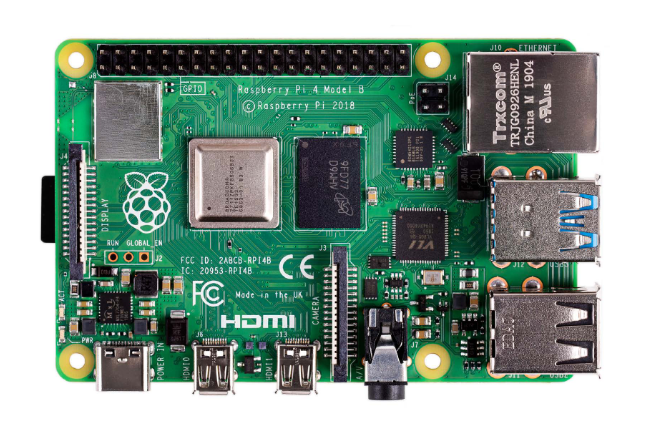
\includegraphics[scale=0.3]{fig5.png}}
	\caption{\textit{Raspberry Pi 4 Model B Board Example}}
	\label{fig5}
\end{figure}

\begin{figure}[htbp]
	\centerline{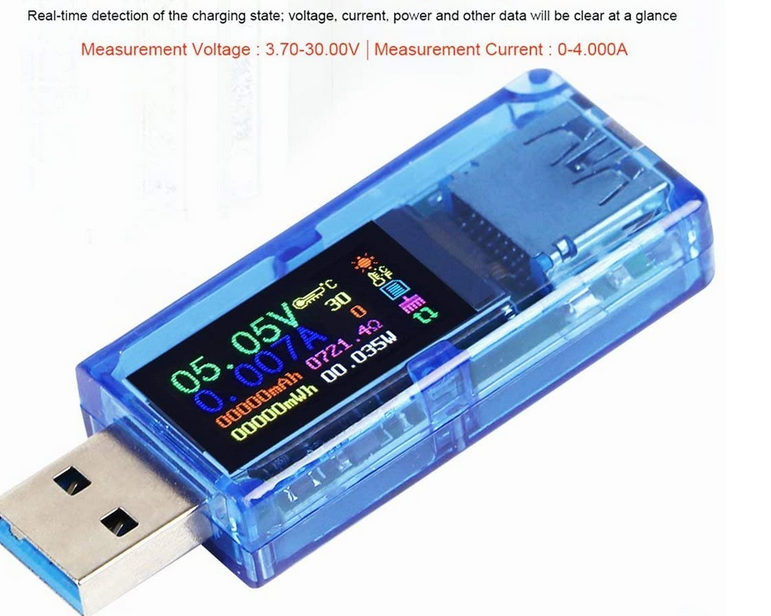
\includegraphics[scale=0.3]{fig6.png}}
	\caption{\textit{MakerHawk USB 3.0 Digital USB Multimeter Sample Display}}
	\label{fig6}
\end{figure}

\section*{Acknowledgment}
We would like to express our deep gratitude to Dr. Yuan Cheng for his support and guidance as advisor to this research. As well, we are grateful to Dr. Ted Krovetz for his wisdom and insight. Finally, we would like to thank Brian A. for generously lending his Raspberry Pi 4B for our research purposes.

\begin{thebibliography}{00}
	\bibitem{1} M. Katagi and S. Moriai, ``Lightweight Cryptography for the Internet of Things,'' \url{https://www.iab.org/wpcontent/IAB-uploads/2011/03/Kaftan.pdf}; 2011.
	\bibitem{2} J.-P. Aumasson, L. Henzen, W. Meier, and M. Naya-Plasencia, ``Quark: A Lightweight Hash,'' in CHES 2010, no. 6225 in LNCS, pp. 1 -15, Springer-Verlag, 2010.
	\bibitem{3} L. Atzori, A. Iera, G. Morabito, ``The Internet of Things: A survey,'' in Comput Netw, 54. pp. 2787-2805, Elsevier, 2010.
	\bibitem{4} N.F. Standard, ``Announcing the advanced encryption standard (AES),'' Federal Information Processing Standards Publication 197 NIST FIPS 197, 2001.
	\bibitem{5} T. Shirai, K. Shibutani, T. Akishita, S. Moriai, and T. Iwata, ``The 128-bit blockcipher CLEFIA,'' in Proceedings of Fast Software Encryption – FSE’07 (A. Biryukov, ed.), no. 4593 in LNCS, pp. 181–195, Springer-Verlag, 2007.
	\bibitem{6} CRYPTREC Lightweight Cryptography WG Members, ``CRYPTREC Cryptographic Technology Guideline (Lightweight Cryptography),'' National Institute of Information and Communication Technology and Information-Technology Promotion Agency, Japan, June 30 2017.

\end{thebibliography}

\end{document}
